\section{Background}\label{sec:background}

In this section, we introduce the concepts and terminology that are necessary to understand the reminder of this paper. First, Section~\ref{sec:sand} introduces some background information about \emph{sandboxes} within the security context. Section~\ref{sec:repackage} presents background information about repackaged application and how they introduce malicious behavior.
Finally, in Section~\ref{sec:android-sandbox} we review the \emph{mining sandbox approach} for detecting repackaged Android apps.

\subsection{The Sandbox approach to ensure security}\label{sec:sand}

A \emph{sandbox} is an isolated environment on an electronic device within which applications cannot affect other programs, the network, or other device data~\cite{DBLP:journals/peerj-cs/MaassSCS16}. Sandbox approach emerged from the need to testing unsafe software, possible malware, without worrying about the integrity of the device under test~\cite{DBLP:conf/esorics/BordoniCS17}, shielding the operation system from any security issue. To ensure safety, sandbox environment should have the minimum requirements to run the program (make sure the program will not escape the sandbox), and make sure it will never assign the program greater privileges than it should have, working with the principle of the \emph{least privilege}. This principle ensures unauthorized access to resources, improving the system's overall health.

Regarding Android ecosystem, the principle of the \emph{least privilege} is ensured by sandbox approach, where apps never access direct resources or data of other apps. Access to sensitives resources like contacts list is granted through specific APIs (Application Programming Interface), which are managed by permissions~\cite{DBLP:journals/corr/abs-2109-06613}. 

The main market source for Android apps is Google Play Store. Unfortunately, it has a flexible policy regarding the process of publishing apps, and therefore, daily many Android apps are removed from the store because of issues related to malware\cite{DBLP:conf/msr/WangLL0X18}. Google Play tries to minimize unauthorized access to sensitive resources by malicious apps, listing each app with its requested permission. Those permissions are presented to Android users at app installation moment since version 6. However, some works presented that most users are careless regarding these permissions since they are only interested to run the app~\cite{DBLP:conf/soups/FeltHEHCW12}. This represents a great security breach since malware usually asks for more permissions than their APIs normally would require~\cite{DBLP:conf/ccs/FeltCHSW11}.

\subsection{Repackage Android app}\label{sec:repackage}

Because of simple bytecode language used~\cite{DBLP:conf/issta/WangGMC15}, Android apps are straight-forward to reverse engineer. Any developers can easily reverse-engineer real apps (benign), modify their contents by inserting malicious code (malware), repackage them with the malicious payloads, and re-advertise them in the official market, Google Play Store, or other markets. Repackage Android apps can leverage the popularity of real apps, to increase its propagation and spread malware.  

It has been raised as a great security problem in Android ecosystem by stakeholders in the app development industry and researchers. There are works~\cite{DBLP:conf/sigmetrics/ViennotGN14} claiming that about 25\% of Google Play Store app content is repackaging apps. Nevertheless, all the workload to detect and remove malware from markets by the stores (official and no official), have not been accurate enough to address the problem as fast as possible. As a result, repackage Android apps follow threatening security and privacy of unsuspicious Android app users, beyond compromising the copyright of the original developer~\cite{DBLP:journals/access/KimLCP19}.

\subsection{Mine Android Sandbox}\label{sec:android-sandbox}

The mine Android sandbox approach~\cite{DBLP:conf/icse/JamrozikSZ16} relies on test generator tools to monitor an Android app's dynamic behavior. The main idea is to explore apps based on their APIs sensitive calls. Thus, sandboxes build upon these APIs calls to create safety rules and then block future calls to other sensitive resources, which diverge from those found in the first exploratory phase. Figure~\ref{fig:mineSandbox} extracted from paper~\cite{DBLP:conf/wcre/BaoLL18}, summarises the approach. 

\begin{figure}[ht]
\centering
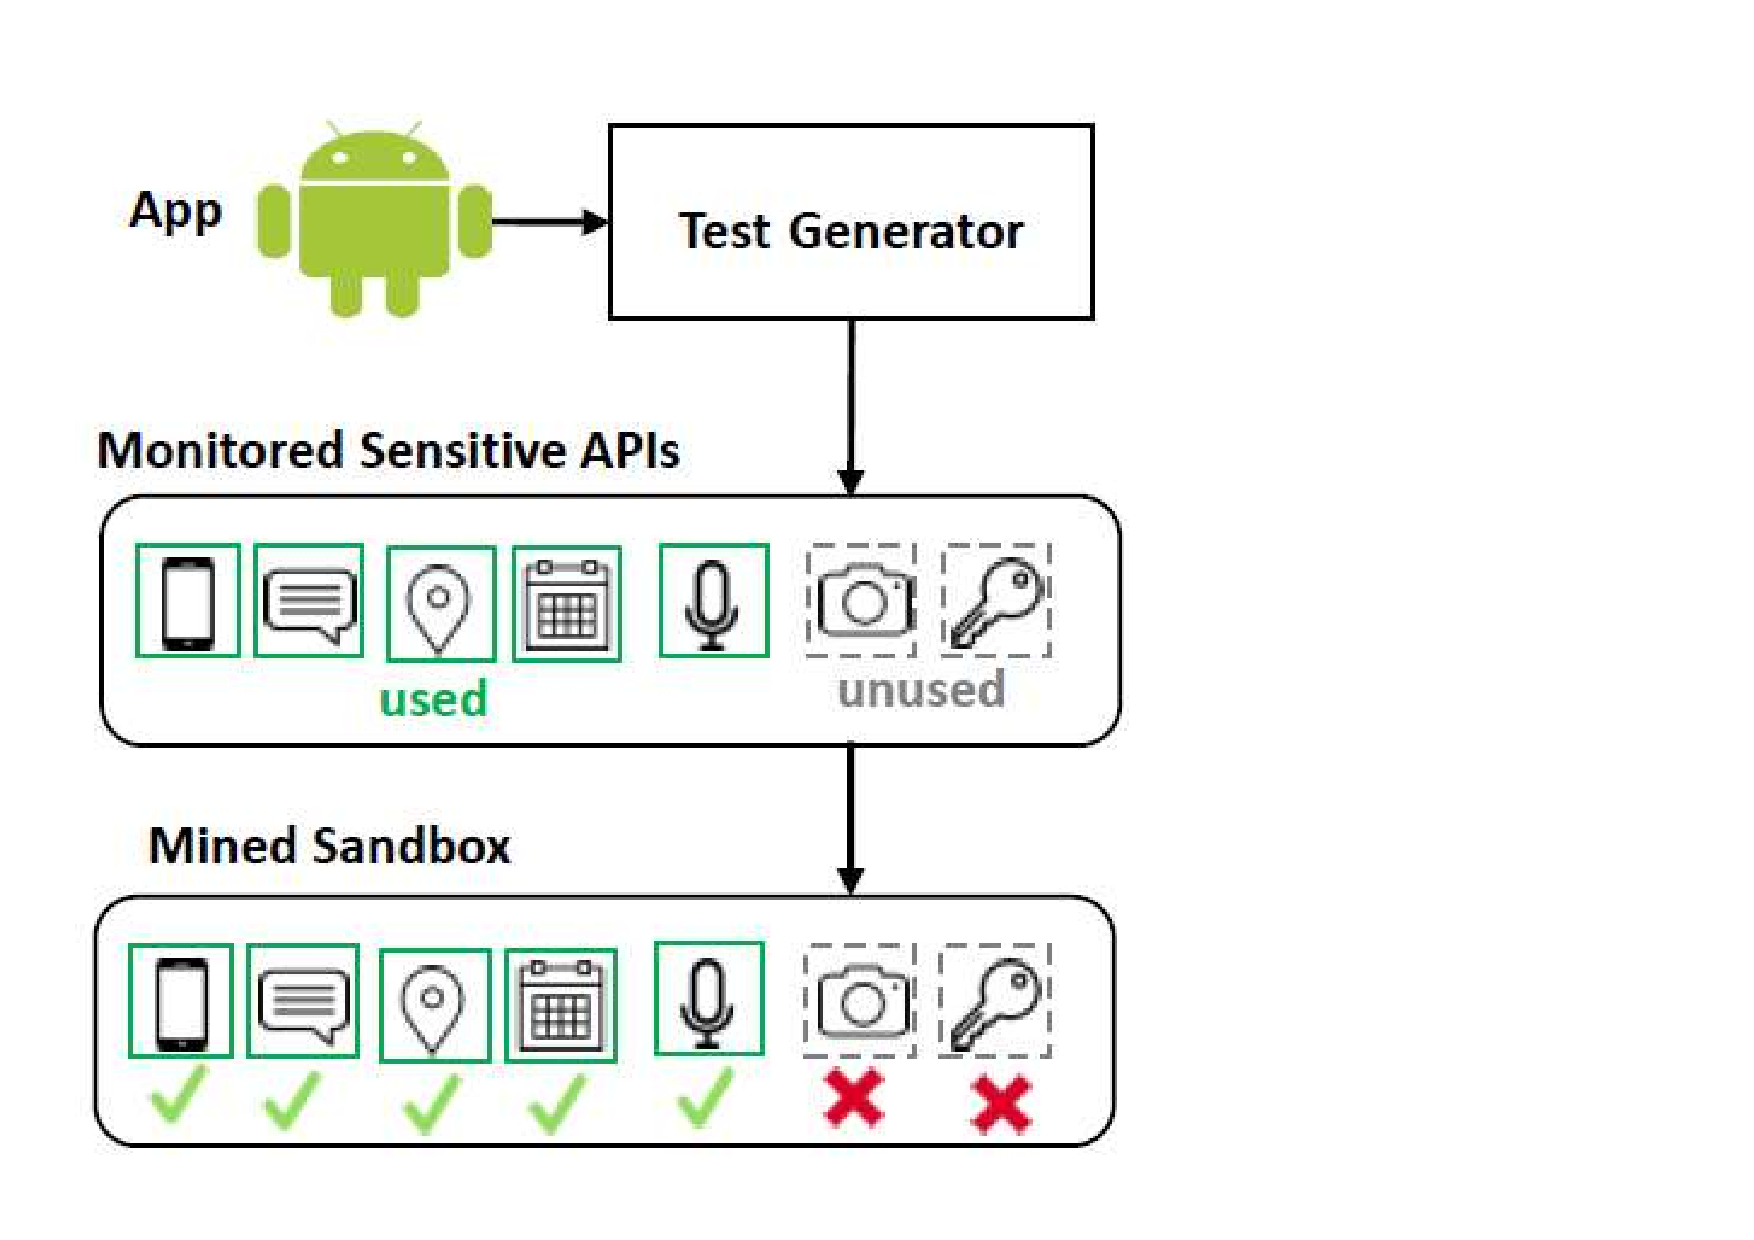
\includegraphics[scale=0.30]{images/mineSandbox.pdf}
\caption{Mine Sandbox. Extracted from~\cite{DBLP:conf/wcre/BaoLL18}}
 \label{fig:mineSandbox}
\end{figure}

The mine Android sandbox approach accuracy suggests a close relationship with the efficiency and exploratory phase. The more efficient the test generator tools (for instance, in terms of code coverage), the more accurate would be the mine sandbox (in terms of repackage/malware identification). There are studies~\cite{DBLP:conf/wcre/BaoLL18,DBLP:conf/scam/CostaMCMVBC20} that explored the effectiveness of mine sandboxes, investigating and comparing the performance of different test generator tools, with diverse exploratory strategies.